\subsection{Komplexität mit TBoxen, obere
Schranke}\label{komplexituxe4t-mit-tboxen-obere-schranke}

\subsubsection{Obere Schranke}

Wir wollen zeigen:

\begin{theorem}
In $\ALC$ ist die Erfüllbarkeit von Konzepten bzgl. TBoxen
\ExpTime-Vollständig.
\end{theorem}

Mit Lemma 2.9: Subsumtion und Äquivalenz \ExpTime-vollständig.

Wir beginnen mit der oberer Schranke (Enthaltensein in \ExpTime):

\begin{itemize}
  \item wir verwenden ein Verfahren aus der Modallogik: Typelimination
  \item basiert auf \emph{syntaktischem} Typ-Begriff
\end{itemize}

\subsubsection{Syntaktische Typen}\label{synt-typ}

Wir nehmen oBdA. an, dass das Eingabe-Konzept $C_0$ in NNF ist und die Eingabe-TBox die Form $\{\top \sqsubseteq C_{\MT}\}$ hat mit $C_{\MT}$ in NNF.

\begin{definition}[Typ]

Ein Typ für $C_{0}$ und $\MT$ ist Teilmenge
$t \subseteq \sub\left( C_{0}, \MT \right)$, so dass

\begin{enumerate}
\item
  $A \in t$ gdw. $\neg A \notin t$ für alle
  $\neg A \in \sub\left( C_{0}, \MT \right)$
\item
  $C \sqcap D \in t$ gdw. $C \in t$ und $D \in t$ für alle
  $C \sqcap D \in \sub\left( C_{0}, \MT \right)$
\item
  $C \sqcup D \in t$ gdw. $C \in t$ oder $D \in t$ für alle
  $C \sqcup D \in \sub\left( C_{0}, \MT \right)$
\item
  $C_{\MT} \in t$
\end{enumerate}
\end{definition}

\begin{tafel}[Beispiel syntaktischer Typ]\label{t:synTyp}

Beispiel:

Sei $C_0 = A$, $\MT = \{\top \sqsubseteq C_{\MT}\}$ mit $$C_{\MT} = \exists r.\exists r.A \sqcap \forall r.A' \sqcap (\neg A \sqcup \neg A')$$

Dann ist $$sub(C_0, \MT) = \{A, C_{\MT}, \exists r.\exists r.A, \forall r.A',\neg A \sqcup \neg A', \exists r.A, A', \neg A, \neg A'\}$$

Sei $M = \{C_{\MT}, \exists r.\exists r. A, \forall r.A', \neg A \sqcup \neg A'\}$

Die Typen für $C_0$ und $\MT$ sind:

\begin{tabular}{ll}
    $t_0 = M \cup \{\neg A, \neg A'\}$ &  $t_0' = M \cup \{ \neg A, \neg A', \exists r.A\}$\\
    $t_1 = M \cup \{\neg A, A'\}$ & $t_1' = M \cup \{\neg A, A', \exists r.A\}$ \\
    $t_2 = M \cup \{A, \neg A'\}$ & $t_2' = M \cup \{A, \neg A', \exists r.A\}$\\
\end{tabular}
\end{tafel}

\subsubsection{Typelimination}\label{typelimination}

Die generelle Idee der Typelimination bei Eingabe $C_0, \MT$:
\begin{itemize}
\item
  Generiere alle Typen für $C_{0}$ und $\MT$ (exponentiell viele)
\item
  Eliminiere wiederholt Typen, die in keinem Modell von $\MT$ vorkommen
  können
\item
  Überprüfe, ob ein Typ überlebt hat, der $C_{0}$ enthält
\item
    Wenn ja, antworte \enquote{erfüllbar}, sonst \enquote{unerfüllbar}
\end{itemize}

\subsubsection{Schlechte Typen}\label{schlechter-typ}

Wir formalisieren \enquote{Typen, die in keinem Modell vorkommen können}.

\begin{definition}[schlechter Typ]\label{def-badtype}

Sei $\Gamma$ Typenmenge und $t \in \Gamma$.

Dann ist $t$ \emph{schlecht in} $\Gamma$, wenn für ein $\exists r.C \in t$ gilt:

\begin{center}Es gibt kein $t^{'} \in \Gamma$ mit
$\left\{ C \right\} \cup \left\{ \text{D\ } \middle| \ \forall r.D \in t \right\} \subseteq t'$.\end{center}
\end{definition}

Erklärung: $t$ braucht einen \enquote{Zeugen}, es gibt aber keinen
geeigneten.

\begin{tafel}[continues=t:synTyp]

    Beispielsweise ist $t_0'$ schlecht in der Menge $\{t_0,t_1,t_2,t_0',t_1',t_2'\}$. Für $\exists r.A \in t_0'$ ist die Menge aus \autoref{def-badtype} $\{A,A'\}$. Kein Typ enhält $A$ und $A'$. Analog: $t_1'$, $t_2'$ sind schlecht. Entfernt man diese drei so erhält man die Menge $\Gamma_1 = \{t_1,t_2,t_2\}$. 

Nun sind aber $\{t_1,t_2,t_3\}$ schlecht in $\Gamma_1$: Sie enthalten $\exists r. \exists r.A$, aber kein Typ in $\Gamma_1$ enthält $\exists r.A$.
\end{tafel}

\begin{algorithmic}
    \Procedure{$\ALC$-Elim}{}
    \State \textbf{input}: $\ALC$-Konzept $C_0$, $\ALC$-TBox $\MT$
    \State \textbf{output}: \enquote{erfüllbar} / \enquote{unerfüllbar}
    \State Berechne $\Gamma_0$: Menge aller Typen für $C_0$ und $\MT$
    \State $i := 0$
    \Repeat
        \State $i := i + 1$
        \State $\Gamma_i := \{ t \in \Gamma_{i - 1} \mid t \text{ nicht schlecht in } \Gamma_{i - 1}\}$
    \Until $\Gamma_i = \Gamma_{i - 1}$
    \If{es gibt $t \in \Gamma_i$ mit $C_0 \in t$}
        \Return \enquote{erfüllbar}
    \Else{}
        \Return \enquote{unerfüllbar}
    \EndIf
    \EndProcedure{}
\end{algorithmic}

\begin{tafel}[continues=t:synTyp]
    Mit dem Beispiel aus T 5.1 enstehen folgende $\Gamma_i$:
    \begin{align*}
        \Gamma_0 &= \{t_0, t_1, t_2, t_0', t_1', t_2'\}\\
        \Gamma_1 &= \{t_0, t_1, t_2\}\\
        \Gamma_2 &= \emptyset
    \end{align*}
\end{tafel}

Wir müssen nun zeigen, dass der Algorithmus
\begin{enumerate}
    \item in exponentieller Zeit terminiert,
    \item korrekt ist,
    \item vollständig ist.
\end{enumerate}

\begin{lemma}
    $\ALC-\texttt{Elim}(C_0,\MT)$ terminiert nach $2^{\text{poly}(|C_0|+|\MT|)}$ Schritten.
\end{lemma}

\begin{proof}
Sei $n = \left| C_{0} \right| + |T|$. Dann gilt:

\begin{enumerate}
\item Es gibt nur $2^{n}$ Typen (\autoref{lem:num-sub} $|\sub(C, \MT)| \leq |C| + |\MT|$)
\item
  In jedem Schritt der repeat-Schleife wird mindestens ein Typ
  eliminiert; die Schleife terminiert nach maximal $2^{n}$
  Durchläufen.
\item
  Die restlichen Operationen (prüfen, ob ein Typ schlecht ist usw.)
  können leicht in Zeit $2^{\text{poly}\left( n \right)}$ implementiert werden.
\end{enumerate}
\end{proof}

\begin{lemma}
    Wenn $\ALC$-Elim($C_0,\MT$) \enquote{erfüllbar} zurückgibt, dann ist $C_0$ erfüllbar bzgl. $\MT$.
\end{lemma}

\begin{proof}
    Wenn der Algorithmus \enquote{erfüllbar} zurückgibt, dann gibt es in der resultierenden Typenmenge $\Gamma_i$ einen Typen $t_0 \in \Gamma_i$ mit $C_0 \in t_0$. Aus $\Gamma_i$ konstruieren wir Interpretation $\MI$ wie folgt:
\begin{align*}
    \Delta^\MI &= \Gamma_{i}\\
    A^\MI &= \{ t \in \Gamma_{i} \mid A \in t \} \text{ für alle Konzeptnamen } A\\
    r^\MI &= \{ (t,t') \mid \forall r.C \in t \text{ impliziert }C \in t' \} \text{ für alle Rollennamen } r
\end{align*} 

\begin{tafel}[Beispiel Modellkonstruktion]\label{t:example51}
    \begin{align*}
        C_0 &= A, \MT = \{ \top \sqsubseteq \forall r.\exists r.A \sqcap(\neg A \sqcup \exists r.A)\}\\
        \sub(C_0, \MT) &= \{ A, C_\MT, \forall r.\exists r.A, \neg A \sqcup \exists r.A, \exists r.A, \neg A\}\\
        M &= \{C_\MT, \forall r.\exists r.A, \neg A \sqcup \exists r.A\}\\
        t_0 &= M \cup \{\neg A\}\\
        t_1 &= M \cup \{\neg A, \exists r.A\}\\
        t_2 &= M \cup \{A, \exists r.A\}\\
    \end{align*}

    \begin{center}
    \begin{tikzpicture}
        \begin{scope}[every node/.style={circle,thick,draw}]
            \node (s1) at (1.5, 2) {$t_0$};
            \node (s2) at (0, 0) {$t_1$};
            \node (s3) at (3, 0) {$t_2$};
        \end{scope}
        \begin{scope}[every node/.style={fill=white}]
            \path [->] (s1) edge node {r} (s2);
            \path [->] (s1) edge node {r} (s3);
            \node at (s3) [right = 1mm of s3] {$A$};
            \path [->] (s2) edge [bend left] node {r} (s3);
            \path [->] (s3) edge [bend left] node {r} (s2);
            \path [->] (s2) edge [loop left] node {r} (s2);
            \path [->] (s3) edge [loop below] node {r} (s3);
        \end{scope}
    \end{tikzpicture}
    \end{center}
\end{tafel}

Die Erfüllbarkeit von $C_0$ bezüglich $\MT$ folgt dann aus:

Behauptung: Für alle $C \in \sub(C_0, \MT)$ und alle $t \in \Gamma_i$ gilt:
\begin{align*}
    C \in t \implies t \in C^\MI
\end{align*}

\begin{tafel}[name=Beweis der Behauptung, continues=t:example51]
    Die Behauptung impliziert das Lemma.
    \begin{enumerate}
        \item Wegen $C_0 \in t_0$ ist $t_0 \in C_0^\MI$
        \item Wegen $C_\MT \in t$ für alle $t \in \Gamma_i$ folgt $t \in C_\MT^\MI$ für alle $t \in \Gamma_i$. Also ist $\MI$ auch Modell von $\MT$.
    \end{enumerate}
    Beweis der Behauptung per Induktion über Struktur von $C$:

\textbf{I.A.}
\begin{itemize}
  \item $t_0 = M \cup \{\neg A\}$
  \item $t_1 = M \cup \{A,\exists r.A\}$
  \item $t_2 = M \cup \{\neg A,\exists r.A\}$
    \item $C = A$. Folgt direkt aus Definition $\MI$.
    \item $C = \neg A$. Wenn $\neg A \in t$, dann ist nach der Definition von Typ (a) $A \notin t$. Nach Definition von $\MI$ ist $t \in {(\neg A)}^\MI$.
\end{itemize}
\textbf{I.S.}
\begin{itemize}
    \item $C = D \sqcap D'$: Wenn $C \in t$, dann ist nach der Definition von  Typ (b) $D, D' \in t$. Nach IV ist $t \in D^\MI$ und $t \in D'^\MI$. Also ist $t$ auch Instanz von ${(D \sqcap D')}^\MI$
    \item $C = D \sqcup D'$: analog.

\item $C = \forall r.D$:
Sei $\forall r.D \in t$ und $\left( t,t' \right) \in r^\MI$. Nach
Definition $r^\MI$ gilt $D \in t'$. Nach I.V.:
$t' \in D^\MI$, also $t \in {( \forall r.D )}^\MI$

\item $C = \exists r.D$:
Sei $\exists r.D \in t$. Da $t \in \Gamma_{i}$ (also nicht
schlecht), gibt es $t' \in \Gamma_{i}$ mit $D \in t'$ und
$E \in t'$ für alle $\forall r.E \in t$. Nach I.V. gilt
$t' \in D^\MI$ und nach Definition von $r^\MI$ gilt
$\left( t,t' \right) \in r^\MI$. Also
$t \in {(\exists r.D )}^\MI$
\end{itemize}
\end{tafel}
\end{proof}


\begin{lemma}
    Wenn $C_0$ bezüglich $\MT$ erfüllbar ist, dann gibt $\ALC-\texttt{Elim}(C_0, \MT)$ \enquote{erfüllbar} zurück.
\end{lemma}

\begin{proof}
    Sei $C_0$ erfüllbar bezüglich $\MT$ und $\MI$ ein Modell von $C_0$ und $\MT$ mit $d_0 \in C_0^\MI$. Sei
    \begin{align*}
        \Gamma = \{ t_\MI(d) \mid d \in \Delta^\MI\}
    \end{align*}
    und $\Gamma_0, \Gamma_1, \ldots \Gamma_k$ die von $\ALC-\texttt{Elim}(C_0, \MI)$ erzeugte Sequenz.
    Wir zeigen:

    Behauptung: $\Gamma \subseteq \Gamma_i$ für alle $i \leq k$.
    \begin{tafel}[Beweis der Behauptung]
    Per Induktion über $i$:

    IA $i = 0$ trivial: jedes Element von $\Gamma$ (semantischer Typ) ist auch syntaktischer Typ (erfüllt a-d).

    IS $i \rightarrow i + 1$: Gelte $\Gamma \subseteq \Gamma_i$, zu zeigen $\Gamma \subseteq \Gamma_{i + 1}$.

    $t \in \Gamma \subseteq \Gamma_i$, es genügt zu zeigen, dass $t$ nicht schlecht in $\Gamma_i$. Sei $\exists r.C \in t$ und $S = \{C\} \cup \{D\mid \forall r.D \in t\}$. Da $t \in \Gamma$, gibt es $d \in \Delta^\MI$ mit $t_\MI(d) = t$. Also gibt es nach Semantik $e \in \Delta^\MI$ mit $(d, e) \in r^\MI$ und $e \in D'$ für alle $D \in S$.

    Es gilt also $S \subseteq t_\MI(e)$ und $t_\MI(e) \in \Gamma \subseteq \Gamma_i$. Also ist $t$ nicht schlecht in $\Gamma_i$.
    \end{tafel}
    Wegen $d_0 \in C_0^\MI$ ist also $C_0 \in t_\MI(d_0) \in \Gamma \subseteq \Gamma_k$. Also gibt der Algorithmus \enquote{erfüllbar} zurück.
\end{proof}


Aus den Lemmas 5.4--5.6 folgt nun:

\begin{theorem}\label{thm:tbox-exptime}
In $\ALC$ ist die Erfüllbarkeit von Konzepten bzgl. TBoxen entscheidbar in \ExpTime.
\end{theorem}

\subsubsection{Zusammenhang mit Tableau-Algorithmen}

Offensichtliche Entsprechungen:

\begin{itemize}
  \item $\sqcap$-Regel, $\sqcup$-Regel, TBox-Regel finden sich wieder in der Definition eines Typs.
  \item $\exists$-Regel und $\forall$-Regel finden sich wieder in Definition von \enquote{schlecht}.
  \item Freiheit von offensichtlichen Widersprüchen findet sich wieder in der Definition eines Typs
\end{itemize}

Unterschiede:

\begin{itemize}
  \item Tableau-Algorithmus benötigt im Worst Case dreifach exponentielle Laufzeit
  \item Typelimination benötigt im Best Case exponentielle Laufzeit
\end{itemize}

\subsection{Komplexität mit TBoxen, untere Schranke}\label{komplexituxe4t-mit-tboxen-untere-schranke}

Um die \ExpTime-Schwere zu zeigen, reduzieren wir auf ein spieltheoretisches Problem:

\subsubsection{ExpTime-Spiele}\label{exptime-spiele}

\begin{itemize}
\item Zwei Spielerinnen spielen auf gegebener aussagenlogischen Formel $\varphi$
\item Jede Variable in $\varphi$ gehört entweder Spielerin 1 oder Spielerin 2
\item Das Spiel beginnt auf einer gegebenen Anfangsbelegung $\pi_0$ der Variablen in $\varphi$.
\item Spielerin 1 beginnt, die Spielerinnen wechseln sich ab.
\item In jedem Zug ändert die jeweilige Spielerin den Wahrheitswert einer ihrer Variablen; es ist erlaubt, zu passen
\item Spielerin 1 gewinnt, wenn $\varphi$ jemals wahr wird (egal, welche Spielerin gezogen hat).
\item Spielerin 2 gewinnt, wenn das Spiel unendlich weitergeht ohne dass $\varphi$ wahr wird
\end{itemize}

\begin{tafel}[Beispiel \ExpTime-Spiele]\mbox{}
    \begin{itemize}
        \item Spiel A: $\varphi = \neg (p_1 \leftrightarrow p_2) \wedge \neg (q_1 \leftrightarrow q_2)$,
            Sp1 kontrolliert $p_1, q_1$, Sp2 kontrolliert $p_2, q_2$. $\pi_0$ macht alle Variablen falsch.

            Sp1 gewinnt wenn $p_1, p_2$ unterschiedlich belegt sind und ebenso $q_1, q_2$. Sp2 gewinnt, wenn sie den letzten Zug von Sp1 immer \enquote{komplementiert}.
            Möglicher Spielverlauf:
            \begin{center}
            \begin{tabular}{rrrrr}
                & $p_1$ & $p_2$ & $q_1$ & $q_2$\\
                & 0 & 0 & 0 & 0\\
                1 & 1 & 0 & 0 & 0\\
                2 & 1 & 1 & 0 & 0\\
                1 & 1 & 1 & 1 & 0\\
                2 & 1 & 1 & 1 & 1\\
            \end{tabular}
        \end{center}

        $\implies$ Sp2 gewinnt.

    \item Spiel B: wie A $\varphi' = \varphi \vee (p_1 \wedge p_2 \wedge q_1 \wedge q_2)$.
        Möglicher Spielverlauf:
            \begin{center}
            \begin{tabular}{rrrrr}
                & $p_1$ & $p_2$ & $q_1$ & $q_2$\\
                & 0 & 0 & 0 & 0\\
                1 & 1 & 0 & 0 & 0\\
                2 & 1 & 1 & 0 & 0\\
                1 & 1 & 1 & 1 & 0\\
            \end{tabular}
        \end{center}
            Bei den möglichen Folge-Kombinationen $1111, 1010, 1110, 0110$ gewinnt Sp1.
    \end{itemize}
\end{tafel}

\begin{definition}[\ExpTime-Spiele]
    Ein \emph{Spiel} ist ein Tupel $\left( \varphi,\ \Gamma_1,\Gamma_2,\pi_{0} \right)$ mit $\Gamma_1,\Gamma_2$ Partitionierung der Variablen in
  $\varphi_1$ und $\pi_{0}$ Anfangsbelegung

    Eine \emph{Konfiguration} ist ein Paar $(i,\pi)$ mit
  $i \in \left\{ 1,2 \right\}$ aktive Spielerin und $\pi$ Belegung

    Eine Belegung $\pi$ ist eine $j$-Variation von $\pi'$ ($j \in \{1, 2\}$), wenn $\pi = \pi'$ oder $\pi$ und $\pi'$ unterscheiden sich nur in einer Variablen $p \in \Gamma_j$.
\end{definition}

\enquote{$\pi$ ist $j$-Variation von $\pi'$} bedeutet: Spielerin $j$ kann
$\pi$ in $\pi'$ transformieren (oder umgekehrt).

Das hier relevante Entscheidungsproblem bezieht sich auf \emph{Gewinnstrategien} für Spielerin 2.

\subsubsection{Gewinnstrategie}\label{definition-5.8-gewinnstrategie}

Intuitiv:

\begin{itemize}
  \item eine Gewinnstrategie sagt Spielerin 2 nach jedem möglichen Spielverlauf wie sie spielen muss um zu gewinnen.
  \item wenn Spielerin 2 eine Gewinnstrategie hat, so kann sie das Spiel immer gewinnen --- egal was Spielerin 1 tut.
\end{itemize}

\begin{definition}[Gewinnstrategie]

Eine  Gewinnstrategie für Spielerin $2$ in Spiel
$\left( \varphi,\Gamma_1,\Gamma_2,\pi_{0} \right)$ ist unendlicher
knotenbeschrifteter Baum $(V,E,\ell)$, wobei $\ell$ jedem Knoten
$v \in V$ Konfiguration $l(v)$ zuweist so, dass

\begin{enumerate}[label={(\alph*)}]
\item Die Wurzel ist beschriftet mit $\left( 1,\pi_{0} \right)$
\item Wenn $\ell\left( v \right) = (2,\pi)$, dann hat $v$ Nachfolger
  $v'$ mit $\ell\left( v' \right) = \left( 1,\pi' \right)$, wobei
  $\pi'$ $2$-Variation von $\pi$.
\item wenn $\ell\left( v \right) = (1,\pi)$, dann hat $v$ Nachfolger
  $v_{0},\ldots,v_{\left| \Gamma_1 \right|}$ mit
  $\ell\left( v_i \right) = (2,\pi_{i})$ wobei
  $\pi_{0},\ldots,\pi_{\left| \Gamma_1 \right|}$ \emph{alle} existierenden
  $1$-Variationen von $\pi$ sind.
\item wenn $\ell\left( v \right) = (i,\pi)$, dann
  $\pi \not\models \varphi$.
\end{enumerate}
\end{definition}

\begin{tafel}[Beispiel Gewinnstrategie]
    Für Spiel A eine Gewinnstrategie für Sp2:
    \begin{center}
    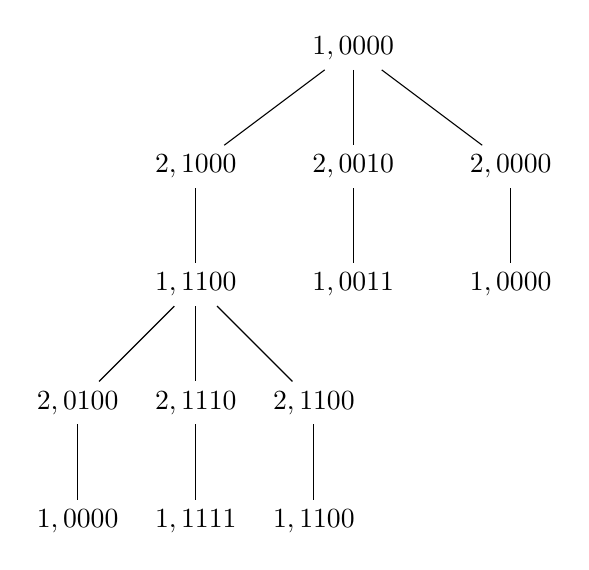
\begin{tikzpicture}
        \begin{scope}[every node/.style={fill=white}]
            \node (s1) at (0, 0) {$1, 0000$};
            \node (s2) at (-2, -1.5) {$2, 1000$};
            \node (s3) at (0, -1.5) {$2, 0010$};
            \node (s4) at (2, -1.5) {$2, 0000$};
            \node (s5) at (-2, -3) {$1, 1100$};
            \node (s6) at (0, -3) {$1, 0011$};
            \node (s7) at (2, -3) {$1, 0000$};
            \node (s8) at (-3.5, -4.5) {$2, 0100$};
            \node (s9) at (-2, -4.5) {$2, 1110$};
            \node (s10) at (-0.5, -4.5) {$2, 1100$};
            \node (s11) at (-3.5, -6) {$1, 0000$};
            \node (s12) at (-2, -6) {$1, 1111$};
            \node (s13) at (-0.5, -6) {$1, 1100$};
        \end{scope}
        \begin{scope}[every node/.style={fill=white}]
            \path [-] (s1) edge (s2);
            \path [-] (s1) edge (s3);
            \path [-] (s1) edge (s4);
            \path [-] (s2) edge (s5);
            \path [-] (s3) edge (s6);
            \path [-] (s4) edge (s7);
            \path [-] (s5) edge (s8);
            \path [-] (s5) edge (s9);
            \path [-] (s5) edge (s10);
            \path [-] (s8) edge (s11);
            \path [-] (s9) edge (s12);
            \path [-] (s10) edge (s13);
        \end{scope}
    \end{tikzpicture}
\end{center}

    In Spiel B gibt es keine Gewinnstrategie für Sp2.
\end{tafel}

\begin{definition}[\ExpTime-Spiel Entscheidungsproblem]
\emph{Spiel\textsubscript{1}} ist das folgende Problem: Gegeben Spiel
$\left( \varphi,\Gamma_1,\Gamma_2,\pi_0 \right)$, entscheide ob
Spielerin 2 eine Gewinnstrategie hat.
\end{definition}

\begin{theorem}[Stockmeyer, Chandra 1979]
Spiel\textsubscript{1} ist \ExpTime-Vollständig
\end{theorem}

Wir wollen nun die \ExpTime-Schwere von Erfüllbarkeit in $\ALC$ bzgl. TBoxen beweisen indem wir Spiel\textsubscript{1} darauf reduzieren.

\subsubsection{Reduktion}\label{reduktion}

Reduziere Spiel\textsubscript{1}: Gegeben Spiel
$\left( \varphi,\Gamma_1,\Gamma_2,\pi_{0} \right)$, konstruiere in
Polynomialzeit Konzept $C_{S}$ und TBox $\MT_{S}$, so dass Spielerin 2 eine Gewinnstrategie in $S$ hat gdw. $C_S$ erfüllbar bezüglich $\MT$ ist.

Idee: (Baum)-Modelle von $C_S$ und $\MT_S$ kodieren Gewinnstrategien.

Sei $\Gamma_1 = \{p_0,\ldots,p_{k - 1}\}$ und $\Gamma_2 = \{p_k, \ldots, p_{n - 1}\}$.

Signatur von $C_S$ und $\MT_S$:
\begin{itemize}
    \item Rollenname $r$ für Kanten im Baum
    \item Konzeptname $W$ für die Wurzel
    \item Konzeptnamen $P_0, \ldots, P_{n - 1}$ für die Variablen
    \item Konzeptnamen $S_1, S_2$ für die aktive Spielerin
    \item Konzeptnamen $V_0, \ldots, V_{n - 1}$ für die Variable, deren Wert zum Erreichen der aktuellen Konfiguration geändert wurde
\end{itemize}

\begin{enumerate}
    \item Die Anfangskonfiguration ist korrekt:
        \begin{align*}
            W \sqsubseteq S_1 \sqcap \bigsqcap_{i < n, \pi_0(p_i) = 0} \neg P_i \sqcap \bigsqcap_{i < n, \pi_0(p_i) = 1} P_i
        \end{align*}
    \item Wenn Spielerin 1 am Zug ist, gibt es $k + 1$ Nachfolger:
        \begin{align*}
            S_1 \sqsubseteq \exists r.(\neg V_0 \sqcap \dots \sqcap \neg V_{n - 1}) \sqcap \bigsqcap_{i < k} \exists r. V_i
        \end{align*}
    \item Wenn Spielerin 2 am Zug ist, gibt es einen Nachfolger:
        \begin{align*}
            S_2 \sqsubseteq \exists r.(\neg V_0 \sqcap \dots \sqcap \neg V_{n - 1}) \sqcup \bigsqcup_{k\leq i < n} \exists r.V_i
        \end{align*}
    \item Es ändert sich höchstens eine Variable pro Zug:
        \begin{align*}
            \top \sqsubseteq \bigsqcap_{i < j < n} \neg (V_i \sqcap V_j)
        \end{align*}
    \item Die ausgewählte Variable ändert ihren Wahrheitswert:
        \begin{align*}
            \top \sqsubseteq \bigsqcap_{i < n}
            \left( \left( P_i \rightarrow \forall r.(V_i \rightarrow \neg P_i)
                    \right) \sqcap \left(
                    \neg P_i \rightarrow \forall r.(V_i \rightarrow P_i)
            \right) \right)
        \end{align*}
    \item Alle anderen Variablen behalten ihren Wert:
        \begin{align*}
            \top \sqsubseteq \bigsqcap_{i < n}
            \left( \left( P_i \rightarrow \forall r.(\neg V_i \rightarrow P_i)
                    \right) \sqcap \left(
                    \neg P_i \rightarrow \forall r.(\neg V_i \rightarrow P_i)
            \right) \right)
        \end{align*}
    \item Die Spielerinnen wechseln sich ab:
        \begin{align*}
            S_1 \sqsubseteq \forall r.S_2, \quad S_2 \sqsubseteq \forall r.S_1, \quad S_1 \sqsubseteq \neg S_2
        \end{align*}
    \item Die Formel $\varphi$ ist immer falsch:
        \begin{align*}
            \top \sqsubseteq \neg \varphi
        \end{align*}
\end{enumerate}
Setze außerdem $C_S = W$. Anmerkung: $C \rightarrow D$ ist Abkürzung für $\neg C \sqcup D$.

\begin{lemma}
    Spielerin 2 hat Gewinnstrategie in $S$ gdw. $C_S$ erfüllbar bezüglich $\MT_S$.
\end{lemma}

\begin{proof}
    \enquote{$\Rightarrow$} Sei $(V, E, \ell)$ eine Gewinnstrategie für Spielerin 2 mit Wurzel $w \in V$. Wir konstruieren Interpretation $\MI$ wie folgt:
    \begin{align*}
        \Delta^\MI = &V, \quad r^\MI = E, \quad W^\MI = \{w\}\\
        P_i^\MI = &\{ v \in V \mid \ell(v) = (t, \pi) \text{ mit } \pi(p_i) = 1\} \quad \text{für alle } i < n\\
        S_i^\MI = &\{v \in V \mid \ell(v) = (i, \pi)\} \quad \text{für alle } i \in \{1, 2\}\\
        V_i^\MI = &\{ v \in V \mid (v', v) \in E \text{ mit } \ell(v') = (t', \pi'),\\
                  &\ell(v) = (t, \pi), \pi(p_i) \neq \pi'(p_i) \} \quad \text{für alle } i < n
    \end{align*}
    Die Erfüllbarkeit von $C_S$ bezüglich $\MT_S$ folgt dann aus:

    Behauptung: $\MI$ ist ein Modell von $W$ und $\MT_S$.
    \begin{tafel}[Teil-Beweis der Behauptung]
        Für die Behauptung zeigen wir exemplarisch, dass $\MI$ die Konzeptinklusion $2$ erfüllt.  Sei $v \in S_1^\MI, \ell(i, \pi)$. Nach Definition von $S_1^\MI$ ist $i = 1$. Nach Bedingung (c) von Gewinnstrategien gibt es $v_0,\ldots,v_k$ mit $\ell(v_i) = (2, \pi_i)$ so dass $\pi_0, \ldots, \pi_k$ alle 1-Variationen von $\pi$ sind. Nach Definition von $r^\MI$ ist $(v, v_i)\in r^\MI$ für alle $i \leq k$. Nach Definition von $V_j^\MI$ gibt es $v_i \in \{v_0\ldots, v_k\}$ mit $v_i \in V_i^\MI$ für alle $i < k$. Ebenfalls gibt es nach Definition $u \in \{v_0, \ldots v_k\}$ mit $i \notin V_0^\MI \cup \dots \cup V_k^\MI$. Also ist $v$ Instanz der rechten Seite der Inklusion $2$. Also ist $\MI$ Modell von $2$.

        Die restlichen Konzeptinklusionen lassen sich analog zeigen.
    \end{tafel}
\end{proof}

\begin{proof}
    \enquote{$\Leftarrow$} Sei $\MI$ ein Modell von $W$ und $\MT_S$. OBdA. ist $\MI$ ein Baummodell. Setze
    \begin{align*}
    V = \Delta^\MI \quad E = r^\MI \quad \ell(v) = (i, \pi) \text{ für alle } v \in V\\
    \text{wobei } i = \begin{cases}
        1 & \text{wenn } v \in S_1^\MI\\
        2 & \text{wenn } v \in S_2^\MI
    \end{cases}
    \text{ und }
    \pi(p_i) = \begin{cases}
        1 & \text{wenn } v \in P_i^\MI\\
        0 & \text{wenn } v \notin P_i^\MI
    \end{cases}
    \end{align*}

    Wegen Konzeptinklusionen (1) und (7) ist $S_1^\MI, S_2^\MI$ eine Partitionierung von $\Delta^\MI$, also ist $\ell$ \emph{wohldefiniert}.
    Noch zu zeigen:

    Behauptung: $(V, E, \ell)$ ist eine Gewinnstrategie für Spielerin 2.

    \begin{tafel}[Beweis der Behauptung]
        Bedingungen einer Gewinnstrategie:
        \begin{enumerate}[label={(\alph*)}]
            \item Gilt nach Nach KI (1) und Definition $(V, E, \ell)$
            \item Sei $\ell(v) = (2, \pi)$. Dann $v \in S_2^\MI$. Nach KI (3) gibt es $v' \in \Delta^\MI$ mit $(v, v') \in r^\MI$ und 
                \begin{itemize}
                    \item $v' \in  (\neg V_0 \sqcap \dots \sqcap \neg V_{n - 1})$ oder
                    \item $v' \in V_i^\MI$ für ein $i \in \{k, \ldots, n - 1\}$
                \end{itemize}
                Im zweiten Fall garantiert zusätzlich KI (4): $v' \notin V_j^\MI$ falls $j \neq i$.

                Sei $\ell(v') = (i', \pi')$. Wegen KIs (5 + 6) ist $\pi'$ eine 2-Variation von $\pi$. Wegen KI (7) ist $v' \in S_1^\MI$, also $i' = 1$.
            \item analog zu (b). Anstelle KI (3) wird KI (2) genutzt.
            \item Nach KI (8).
        \end{enumerate}
    \end{tafel}
\end{proof}

Daraus folgt:
\begin{theorem}
In $\ALC$ ist die Erfüllbarkeit von Konzepten bezüglich TBoxen \ExpTime-schwer.
\end{theorem}

Daraus ergibt sich zusammen mit \autoref{thm:tbox-exptime}:
%TODO: repeat theorem 5.1

\subsection{Komplexität ohne TBoxen obere
Schranke}\label{komplexituxe4t-ohne-tboxen-obere-schranke}

Wir wollen zeigen:

\begin{theorem}
In $\ALC$ ist die Erfüllbarkeit von Konzepten (ohne TBoxen)
\PSpace-Vollständig.
\end{theorem}
Mit \autoref{lem:problem-reduction} sind dann auch Subsumtion und Äquivalenz \PSpace-vollständig.

Wir beginnen mit der oberen Schranke (Enthaltensein in \PSpace) und benutzen dazu ein Verfahren aus der Modallogik: \emph{K-Worlds}.

Zur Erinnerung: Wenn Konzept $C$ erfüllbar ist, dann hat $C$ ein Baummodell (\autoref{thm:baummodell}). Mit TBox $\MT$ kann es sein, dass alle Baummodelle unendlich sind, z.B. $A$ erfüllbar bezüglich $\MT = \{A \sqsubseteq \exists r.A\}$. Ohne TBox gibt es stets ein Baummodell, dessen Tiefe durch $|C|$ beschränkt ist. Es genügt die Existenz solcher Modelle zu überprüfen.

\subsubsection{\texorpdfstring{$\ALC$}{ALC}-Worlds}\label{alc-worlds}

Gesucht: Ein Algorithmus, der in \PSpace{} läuft, aber:
\begin{itemize}
\item Ein linear tiefer Baum ist exponentiell groß.
\item Wenn wir gesamtes Modell im Speicher hielten, dann würde das exponentiellen Platz erfordern.
\item Stattdessen: Prüfe Existenz des Baumes mittels Tiefensuche; halte zu
  jeder Zeit nur einen Pfad des Baumes im Speicher.
\end{itemize}

Wir entwickelt einen nichtdeterministischen Algorithmus, da
\begin{theorem}[Savitch 1970]
    \PSpace{} $=$ \NPSpace{}
\end{theorem}

Wir nehmen an, dass die Eingabe $C_0$ in NNF ist. Weiterhin verwenden wir wieder Typen, definieren diese jedoch differenzierter.

\begin{definition}[$i$-Konzepte]

Für $i \geq 0$ ist die Menge der $i$-Konzepte definiert als:
\begin{align*}
\sub_{i} \left( C_0 \right) = \left\{ C \in \sub\left( C_0 \right) \mid \rd\left( C \right) \leq i \right\}
\end{align*}
\end{definition}
$\rd(C)$ ist die Rollentiefe eines Konzepts.
(Siehe \autoref{sec:def-rollentiefe})

\begin{definition}[$i$-Typ]
Sei $i \geq 0$.

$i$-Typ für $C_{0}$ ist Teilmenge
$t \subseteq \sub_{i}\left( C_{0} \right)$, so dass

\begin{enumerate}
\item
  $A \in t$ gdw. $\neg A \notin t$ für alle
  $\neg A \in \sub_{i}\left( C_{0} \right)$
\item
  $C \sqcap D \in t$ gdw. $C \in t$ und $D \in t$ für alle
  $C \sqcap D \in \sub_{i}\left( C_{0} \right)$
\item
  $C \sqcup D \in t$ gdw. $C \in t$ oder $D \in t$ für alle
  $C \sqcup D \in \sub_{i}\left( C_{0} \right)$
\end{enumerate}
\end{definition}

\begin{tafel}[Beispiel $i$-Typen]\label{t:example58}
    Sei $C_0 = A \sqcap \exists r.B \sqcap \exists r. \neg B \sqcap \forall r.\exists r.\neg A$
    \begin{align*}
        \sub(C_0) &=
        \{ \underbrace{A, B, \neg A, \neg B}_{0-\text{Konzepte}}
            \underbrace{\exists r.B, \exists r.\neg B, \exists r.\neg A}_{1-\text{Konzepte}}
            \underbrace{\forall r.\exists r.\neg A, C_0}_{2-\text{Konzepte}}
        \}\\
        \rd(C_0)& = 2
    \end{align*}
    Beispiele für $i$-Typen $i \leq 2$ sind:
    \begin{itemize}
        \item 0-Typ: $\{A, \neg B\}$
        \item 1-Typ: $\{A,  B, \exists r.B\}$
        \item 2-Typ: $\{A,  \neg B, \exists r.B, \forall r. \exists r \neg A\}$
    \end{itemize}
\end{tafel}

\begin{algorithmic}
    \Procedure{$\ALC$-Worlds}{$C_0$}
    \State{} $i\gets \rd(C_0)$
    \State{} Rate $t \subseteq \sub_i(C_0)$ mit $C_0 \in t$
    \State{} \Call{recurse}{$t, i, C_0$}
    \EndProcedure{}
    
    \Procedure{recurse}{$t, i, C_0$}
    \If{$t$ ist kein $i$-Typ für $C_0$} \Return{} \texttt{false}\EndIf
    \ForAll{$\exists r.C \in t$}
        \State{} $S:= \{C\} \cup \{D \mid \forall r.D \in t\}$
        \State{} Rate $t' \subseteq \sub_{i - 1}(C_0)$ mit $S \subseteq t'$
        \If{\Call{recurse}{$t', i - 1, C_0$} = \texttt{false}} \Return \texttt{false} \EndIf
    \EndFor
    \Return \texttt{true}
    \EndProcedure{}
\end{algorithmic}

\begin{tafel}[name=Beispiel $\ALC$-Worlds, continues=t:example58]
    $\ALC-\text{Worlds}(C_0)$ hat einen erfolgreichen Lauf.

    \begin{center}
    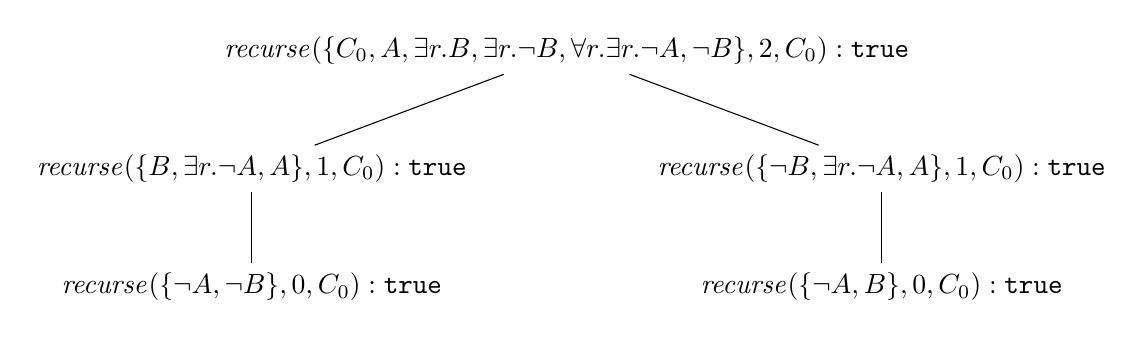
\begin{tikzpicture}
        \begin{scope}[every node/.style={fill=white}]
            \node (s1) at (0, 0) {$
                \mathit{recurse}(\{C_0, A, \exists r.B, \exists r.\neg B, \forall r.\exists r. \neg A, \neg B\}, 2, C_0) : \texttt{true}
             $};
            \node (s2) at (-4, -1.5) {$
                \mathit{recurse} (\{B, \exists r.\neg A, A\}, 1, C_0) : \texttt{true}
            $};
            \node (s3) at (4, -1.5) {$
                \mathit{recurse} (\{\neg B, \exists r.\neg A, A\}, 1, C_0) : \texttt{true}
            $};
            \node (s4) at (-4, -3) {$
                \mathit{recurse} (\{\neg A, \neg B\}, 0, C_0) : \texttt{true}
            $};
            \node (s5) at (4, -3) {$
                \mathit{recurse} (\{\neg A, B\}, 0, C_0) : \texttt{true} 
            $};
        \end{scope}
        \begin{scope}[every node/.style={fill=white}]
            \path [-] (s1) edge (s2);
            \path [-] (s1) edge (s3);
            \path [-] (s2) edge (s4);
            \path [-] (s3) edge (s5);
        \end{scope}
    \end{tikzpicture}
    \end{center}
\end{tafel}

Wir müssen nun zeigen, dass der Algorithmus
\begin{enumerate}
    \item terminiert und nur polynomiellen Platz benötigt,
    \item korrekt ist und
    \item vollständig ist.
\end{enumerate}

Wir beginnen wieder mit Terminierung und Komplexitätsanalyse.

\begin{lemma}
    $\ALC-\texttt{Worlds}(C_0)$ terminiert und benötigt polynomiellen Platz (in $|C_0|$).
\end{lemma}

\begin{proof}
    Jeder Lauf von $\ALC-\texttt{Worlds}(C_0)$ kann als Rekursionsbaum $B = (V, E, \ell)$ dargestellt werden:
    \begin{itemize}
        \item Wurzel: initialer Aufruf von \texttt{recurse}, übrige Knoten: rekursive Aufrufe
        \item $(v, v') \in E$ wenn Aufruf $v'$ während Aufruf $v$ stattfindet
        \item $\ell(v) = (p_1(v), p_2(v), p_3(v))$ sind Parameter bei Aufruf $v$
    \end{itemize}
    Nun ist leicht zu sehen, dass der Verzweigungsgrad von $B$ beschränkt ist durch die Anzahl an Subkonzepten $\exists r.C$ von $C_0$ also durch $|C_0|$. Außerdem ist die Tiefe von $B$ beschränkt durch $\rd(C_0)$, also durch $|C_0|$.
    Also terminiert $\ALC-\texttt{Worlds}(C_0)$ und
    \begin{itemize}
        \item Rekursionsstapel hat Tiefe $\leq |C_0|$ und
        \item Speicherbedarf pro Aufruf polynomiell in $|C_0|$.
    \end{itemize}
    Also wird nur polynomiell viel Platz benötigt.
\end{proof}

\begin{lemma}
    $\ALC-\texttt{Worlds}(C_0)$ = \texttt{true}, dann ist $C_0$ erfüllbar
\end{lemma}

\begin{proof}
    Sei $\ALC-\texttt{Worlds}(C_0) = $ \texttt{true} und $T = (V, E, \ell)$ der Rekursionsbaum eines erfolgreichen Laufen mit Wurzel $v_0$. Für jeden Knoten $v \in V \setminus \{v_0\}$ sei $\sigma(v)$ der Rollenname $r$ des Konzeptes $\exists r.C$, für das der Aufruf $v$ gemacht wurde. Aus B konstruieren wir Interpretation $\MI$ wie folgt:
    \begin{align*}
        \Delta^\MI &= V\\
        r^\MI &= \{(v, v') \in E \mid \sigma(v') = r\} \quad \text{für alle Rollennamen } r\\
        A^\MI &= \{v \mid A \in p_1(v)\} \quad \text{für alle Konzeptnamen } A\\
    \end{align*}
    ($p_1(v)$ erster Parameter in $\ell(v)$)

    Behauptung: Für alle $C \in \sub(C_0)$ und $v \in V : C \in p_1(v) \implies v \in C^\MI$. (Beweis der Behauptung in der Übung)

    Da $C_0 \in p_1(v_0)$, ist auch $v_0 \in C_0^\MI \implies \MI$ ist Modell von $C_0$.
\end{proof}


\begin{lemma}
    Wenn $C_0$ erfüllbar ist, dann gibt es einen Lauf von 
    $\ALC-\texttt{Worlds}(C_0)$, der \texttt{true} zurückgibt.
    \begin{proof}
        Sei $C_0$ erfüllbar und $\MI$ ein Modell von $C_0$ mit $d_0 \in C_0^\MI$. Für jedes $d \in \Delta^\MI$ und $i \geq 0$ definiere:
        \begin{align*}
            t_i(d) = \{C \in \sub_i(C_0) \mid d \in C^\MI\}
        \end{align*}
        Idee: Wir verwenden $\MI$, um die nichtdeterministischen Entscheidungen von $\ALC-\texttt{Worlds}(C_0)$ zu einem erfolgreichen Lauf zu \enquote{lenken}. Zu diesen Zweck übergeben wir eine Element $d \in \Delta^\MI$ als virtuelles viertes Argument $p_4$ an \texttt{recurse}, so dass für alle $v \in V$:
        \begin{align*}
             \tag{*}
             \label{eqn:alc-worlds-impl}
            C \in p_1(v) \implies p_4(v) \in C^\MI
        \end{align*}
        \begin{tafel}[Vorgehen im Detail]\mbox{}
            \begin{itemize}
                \item Der erste Rateschritt rät $t_i(d_0)$ mit $i = \rd(C_0)$,
                    im ersten Aufruf von \texttt{recurse} ist $p_4(v_0) = d_0$, offenbar ist \eqref{eqn:alc-worlds-impl} erfüllt.
                \item Wenn die forall-Schleife von \texttt{recurse}$(t_i, i, C_0, d)$ das Konzept $\exists r.C$ bearbeitet, wähle ein $d' \in \Delta^\MI$ mit $(d, d') \in r^\MI$ und $d' \in D$ für alle $D \in S$ ($S$ aus dem Algorithmus). So ein $d'$ existiert wegen der Bedingung \eqref{eqn:alc-worlds-impl}. Wähle $t_{i - 1}(d')$ im Rateschritt und verwende $d'$ als $p_4(v')$ im Folgenden rekursiven Unteraufruf (Wieder ist \eqref{eqn:alc-worlds-impl} erfüllt). Da alle geratenen Mengen $i$-Typen sind, ist der Lauf erfolgreich.
            \end{itemize}
        \end{tafel}
    \end{proof}
\end{lemma}

Aus Lemmas 5.18--5.20 folgt nun:
\begin{theorem}\label{thm:alc-pspace}
    In $\ALC$ ist die Erfüllbarkeit von Konzepten (ohne TBoxen) entscheidbar in \PSpace.
\end{theorem}

\subsubsection{\texorpdfstring{$\ALC$}{ALC}-Worlds vs. Tableau-Algorithmen}
Offensichtliche Entsprechungen:
\begin{itemize}
  \item $\sqcap$-Regel, $\sqcup$-Regel finden sich wieder in der Definition eines $i$-Typs.
  \item $\exists$-Regel und $\forall$-Regel finden sich wieder im rekursiven Aufruf.
  \item Freiheit von offensichtlichen Widersprüchen findet sich wieder in der Definition eines $i$-Typs
  \item Korrektheitsbeweise sich recht ähnlich
\end{itemize}

Unterschiede:

\begin{itemize}
    \item Tableau-Algorithmus ist deterministisch; hat dafür aber \enquote{teure} $\sqcup$-Regel.
    \item Tableau-Algorithmus ist nicht platzoptimiert.
\end{itemize}

$\ALC$-Worlds kann auf $\ALCI, \ALCQ, \ALCQI$ erweitert werden. Auch in diesen Logiken ist Erfüllbarkeit ohne TBoxen in \PSpace.

\subsection{Komplexität ohne TBoxen untere
Schranke}\label{komplexituxe4t-ohne-tboxen-untere-schranke}

Wir reduzieren wieder ein spieltheoretisches Problem, um \PSpace-Schwere zu zeigen.


\subsubsection{PSpace-Spiele}

\begin{itemize}
    \item Zwei Spielerinnen spielen auf gegebener aussagenlogischen Formel $\varphi$.
    \item Jede Variable in $\varphi$ gehört entweder Spielerin 1 oder Spielerin 2. Jeder Spielerin gehören \emph{gleich viele Variablen}. Die Variablen der Spielerinnen sind linear geordnet.
    \item Spielerin 1 beginnt, die Spielerinnen wechseln sich ab.

    \item In jedem Zug wählt Spielerin Wahrheitswert ihrer nächsten Variable.

    \item Spielerin 1 gewinnt, wenn $\varphi$ am Ende wahr ist; sonst gewinnt Spielerin 2.
\end{itemize}

\begin{tafel}[Beispiel \PSpace-Spiel]
    \begin{align*}
        \varphi = \neg p_1 \rightarrow p_2 \wedge (\neg p_2 \rightarrow (p_4 \rightarrow \neg p_3))
    \end{align*}
    $p_1, p_3$ gehören $P_1$, $p_2, p_4$ gehören $P_2$.
    \begin{enumerate}
        \item $p_1 = 1$ (sonst gewinnt $P_2$ mit $p_2$ = 0)
        \item $p_2 = 0$ (um 2. Implikation zu \enquote{aktivieren})
        \item $p_3 = 0$
        \item $p_4 = 0$
    \end{enumerate}
    $1000$ erfüllt $\varphi \implies$ Spielerin $1$ gewinnt.
\end{tafel}

Unterschiede zu \ExpTime-Spielen:
\begin{itemize}
    \item Das Spiel endet immer; die Anzahl an Schritten ist vorbestimmt.
    \item Die Spielerin hat keine Freiheit in der Wahl ihrer Variablen.
    \item Jede Variable bekommt nur einmal einen Wahrheitswert zugewiesen.
    \item Man darf nicht passen.
    \item Es wird keine Anfangsbelegung benötigt.
\end{itemize}

\begin{definition}[\PSpace-Spiel]
Ein \emph{Spiel} ist eine aussagenlogische Formel $\varphi$ mit Variablen
  $p_1,\ldots,p_{n}$, $n$ geradzahlig.

  Eine \emph{Konfiguration} ist ein Wort $w \in {\left\{ 0,1 \right\}}^*$
\end{definition}

\begin{itemize}
    \item Variablen $p_i$ mit $i$ ungerade gehören Spielerin 1, die anderen Spielerin 2.
    \item Konfiguration $w$ ist partielle Belegung: $i$-tes Symbol ist Wahrheitswert von $p_i$.
\end{itemize}

Das hier relevante Entscheidungsproblem bezieht sich auf Gewinnstrategien für Spielerin 1.

\begin{definition}[Gewinnstrategie]

Gewinnstrategie für Spieler 1 in Spiel $\varphi$ ist endlicher
knotenbeschrifteter Baum $(V,E,\ell)$, wobei $\ell$ jedem Koten
$v \in V$ Konfiguration $\ell(v)$ zuweist, so dass
\end{definition}
\begin{enumerate}[label={(\alph*)}]
\item
  Wurzel beschriftet mit $\varepsilon$ (leere Konfiguration).
\item
  wenn $\ell\left( v \right) = w$ mit $\left| w \right|$ gerade und
  $\left| w \right| < n$ (Also Spielerin 1 am Zug), dann hat $v$
  Nachfolger $v'$ mit $\ell\left( v' \right) \in \{ w0,w1\}$.
\item
  wenn $\ell\left( v \right) = w$ mit $|w|$ ungerade
  (also Spieler 2 am Zug), dann hat $v$ Nachfolger $v'$ und
  $v''$ mit $\ell\left( v' \right) = w0$ und
  $\ell\left( v'' \right) = w1$.
\item
  wenn $\ell\left( v \right) = w$ mit $\left| w \right| = n$, dann
  $w \models \varphi$.
\end{enumerate}

\begin{tafel}[Beispiel \PSpace{} Gewinnstrategie]\mbox{}
    \begin{center}
    \begin{tikzpicture}
        \begin{scope}[every node/.style={fill=white}]
            \node (s1) at (0, 0) {$\varepsilon$};
            \node (s2) at (0, -1) {$1$};
            \node (s3) at (2, -2) {$10$};
            \node (s4) at (-2, -2) {$11$};
            \node (s5) at (2, -3) {$100$};
            \node (s6) at (-2, -3) {$111$};
            \node (s7) at (1, -4) {$1000$};
            \node (s8) at (3, -4) {$1001$};
            \node (s9) at (-3, -4) {$1110$};
            \node (s10) at (-1, -4) {$1111$};
        \end{scope}
        \begin{scope}[every node/.style={fill=white}]
            \path [-] (s1) edge (s2);
            \path [-] (s2) edge (s3);
            \path [-] (s2) edge (s4);
            \path [-] (s3) edge (s5);
            \path [-] (s4) edge (s6);
            \path [-] (s5) edge (s7);
            \path [-] (s5) edge (s8);
            \path [-] (s6) edge (s9);
            \path [-] (s6) edge (s10);
        \end{scope}
    \end{tikzpicture}
    \end{center}
\end{tafel}

\begin{definition}[\PSpace-Spiel Entscheidungsproblem]
    Spiel\textsubscript{2} ist das folgende Problem: Gegeben Spiel $\varphi$, entscheide, ob Spielerin 1 eine Gewinnstrategie hat.
\end{definition}

\begin{theorem}[Schaefer 1978]
    Spiel\textsubscript{2} ist \PSpace-vollständig.
\end{theorem}

Wir beweisen \PSpace-Schwere von Erfüllbarkeit in $\ALC$ ohne TBoxen per Reduktion von Spiel\textsubscript{2}.

\subsubsection{Reduktion}

Ziel: Gegeben Spiel $\varphi$, konstruieren (in Polynomialzeit) Konzept $C_\varphi$, so dass Spielerin eine Gewinnstrategie in $\varphi$ hat gdw. $C_\varphi$ erfüllbar ist.

Idee: Modelle von $C_\varphi$ kodieren Gewinnstrategien.

Die Variablen in $\varphi$ seien $p_1, \ldots, p_n$, n geradzahlig.

Signatur von $C_\varphi$:
\begin{itemize}
    \item Rollenname $r$ für Kanten im Baum
    \item Konzeptnamen $P_1, \ldots, P_n$ für die Wahrheitswerte der Variablen in partiellen Belegungen.
\end{itemize}
Wir schreiben $\forall r^i.C$ für $\underbrace{\forall r.\ldots\forall r.}_{i-\text{mal}}C$.

$C_\varphi$ ist eine Konjunktion mit folgenden Konjunkten.

\begin{enumerate}
    \item $|w|$ ist gerade gdw. Spielerin 1 am Zug gdw. Knoten auf Tiefe $i, 2|i$. Dann gibt es einen Nachfolger, der Wert für $P_{i + 1}$ auswählt.
        \begin{align*}
            C_1 := \bigsqcap_{i \in \{0, 2, \ldots, n - 2\}}
            \forall r^i.(\exists r.\neg P_{i + 1} \sqcup \exists r.P_{i + 1})
        \end{align*}
    \item $|w|$ ungerade gdw. Spielerin 2 am Zug gdw. Knoten auf Tiefe $i, 2 \not| i$. Dann gibt es zwei Nachfolger für beide Werte von $P_{i + 1}$.
        \begin{align*}
            C_2 := \bigsqcap_{i \in \{1, 3, \ldots, n - 1\}} 
            \forall r^i.(\exists r.\neg P_{i + 1} \sqcap \exists r.P_{i + 1})
        \end{align*}
    \item Einmal gewählte Wahrheitswerte bleiben erhalten:
        \begin{align*}
            C_3 := \bigsqcap_{1 \leq i \leq j < n} \forall r^j.\left( \left (
                    P_i \rightarrow \forall r.P_i
                    \right) \sqcap \left(
                    \neg P_i \rightarrow \forall r. \neg P_i
                \right)\right)
        \end{align*}
    \item An den Blättern ist $\varphi$ wahr:
        \begin{align*}
            C_4 := \forall r^n.\varphi
        \end{align*}
\end{enumerate}

Setze $C_\varphi = C_1 \sqcap C_2 \sqcap C_3 \sqcap C_4$.

\begin{lemma}
    Spielerin 1 hat Gewinnstrategie in $\varphi$ gdw. $C_\varphi$ erfüllbar ist.
\end{lemma}

Daraus folgt:

\begin{theorem}
    In $\ALC$ ist die Erfüllbarkeit von Konzepten (ohne TBoxen) \PSpace-schwer.
\end{theorem}

Daraus und aus \autoref{thm:alc-pspace} folgt:
%TODO repeat theorem 5.14

\subsubsection{Gründe für Entscheidbarkeit?}

Es gab eine Zeitlang Diskussionen darüber, was die beste Erklärung für die Entscheidbarkeit von Modal- und Beschreibungslogiken ist.
\begin{itemize}
    \item Existenz von Baummodellen
    \item Einbettbarkeit in das 2-Variablen-Fragment der Prädikatenlogik
    \item Einbettbarkeit in das Guarded Fragment der Prädikatenlogik.
\end{itemize}

\subsection{Unentscheidbare Erweiterungen}\label{unentscheidbare-erweiterungen}

Einige Erweiterungen von $\ALC$, die zunächst vielleicht harmlos erscheinen, können zu \emph{Unentscheidbarkeit} führen. Wir betrachten hier beispielhaft konkrete Bereiche, die es erlauben Zahlen, Strings und anderen Datentypen zu verwenden.

\subsubsection{Konkrete Bereiche}

\begin{definition}[Konkreter Bereich]
    Ein konkreter Bereich ist ein Paar $\MB = (\Delta^\MB, \Phi^\MB)$, wobei
\begin{itemize}
    \item $\Delta^\MB$ eine Menge von \emph{Werten} ist und
    \item $\Phi^\MB$ eine Menge von \emph{Prädikaten}
\end{itemize}
so dass jedes $P \in \Phi^\MB$ mit einer Stelligkeit $n \geq 0$
ausgestattet ist und mit einer Extension
$P^\MB \subseteq {\left( \Delta^\MB \right)}^n$.
\end{definition}

\begin{tafel}[Beispiel konkrete Bereiche]\mbox{}
    \begin{itemize}
        \item Beispiel 1 $\MB_\Q = \left( \Delta^{\MB_\Q}, \Phi^{\MB_\Q} \right)$: 
            \begin{align*}
                \Delta^{\MB_\Q} &= \Q\\
                \Phi^{\MB_\Q} &= \{ =_q \mid q \in \Q \} \cup \{+, -\}\\
                {(=_q)}^{\MB_\Q} &= \{(q)\} \quad \text{für alle } q \in \Q\\
                +^{\MB_\Q} &= \{(q_1, q_2, q_3) \mid q_1 + q_2 = q_3\}\\
                -^{\MB_\Q} &= \{(q_1, q_2, q_3) \mid q_1 - q_2 = q_3\}
            \end{align*}
        \item Beispiel 2 $\MB_S = \left( \Delta^{\MB_S}, \Phi^{\MB_S} \right)$: 
            \begin{align*}
                \Delta^{\MB_S} &= \text{Menge aller Wörter über Unicode 2.0}\\
                \Phi^{\MB_S} &= \{ =_s \mid s\ \text{ist Unicode-Wort}\} \cup \{\text{concat}\}\\
                {(=_s)}^{\MB_S} &= \{(s)\}\ \text{für alle}\ s\\
                \text{concat}^{\MB_S} &= \{(s_1, s_2, s_3) \mid s_1 \cdot s_2 = s_3\}
            \end{align*}
    \end{itemize}
\end{tafel}


\begin{definition}[$\ALCB$ Syntax]
    Sei $\MB$ ein konkreter Bereich. $\ALCB$ ist die Erweiterung von $\ALC$ um $\MB$, d.h.\ um
    \begin{itemize}
\item \emph{Featurenamen} (eine zusätzliche Art von Rolle) und
\item die Konstruktoren $\exists R_1, \ldots, R_n.P$ und
  $\forall R_1,\ldots,R_n.P$
\end{itemize}
wobei $P \in \Phi^\MB$ $n$-stellig ist und die $R_i$
\emph{Rollenkomposition} der Form $$r_1;\ldots;r_{k};f$$ sind mit
$r_{j}$ Rollenname und $f$ Featurename.
\end{definition}

\begin{tafel}[Beispiel $\ALCB$ Syntax]
    \begin{align*}
        \text{Mensch} &\sqsubseteq \forall \overbrace{\text{alter}}^\text{Featurename},\overbrace{\text{eltern}}^\text{Rolle};\overbrace{\text{alter}}^\text{Featurename}.<\\
        \text{KGE} &\equiv \text{Mensch} \sqcap \forall \text{mutter};\text{alter},\text{vater};\text{alter}.=\\
        \text{NAK} &\equiv \text{Mensch} \sqcap \exists \text{alter}, \text{geschwister};\text{alter}.<
    \end{align*}
\end{tafel}

\begin{definition}[$\ALCB$ Semantik]
Eine Interpretation $\MI$ ordnet nun zusätzlich zu jedem Featurenamen
$f$ eine Funktion $f^\MI:\Delta^\MI \rightarrow \Delta^\MB$ zu. Für
jede Rollenkomposition $$R = r_1;\ldots;r_k;f$$ bezeichnet $R^\MI$
die Komposition der Interpretationen:
$$R^\MI = r_1^\MI \circ \cdots \circ r_k^\MI \circ f^\MI$$

Die Semantik der zusätzlichen Konstruktoren ist nun:
    \begin{multline*}
        {( \exists R_1,\ldots, R_k.P )}^\MI =\\
    \left\{ d \in \Delta^\MI \mid \exists d_1,\ldots,d_k: ( d,d_i) \in R_i^\MI\ \text{für}\ 1 \leq i \leq k\ \text{und}\ ( d_1, \ldots, d_k ) \in P^\MB \right\}
    \end{multline*}
    \begin{multline*}
    {( \forall R_1,\ldots, R_k.P )}^\MI =\\
                  \left\{ d \in \Delta^\MI \mid \forall d_1,\ldots,d_k:( d,d_i) \in R_i^\MI\ \text{für}\ 1 \leq i \leq k\ \text{impliziert}\ (d_1, \ldots, d_k) \in P^\MB \right\}
\end{multline*}
%Holy f*ck batman, aligning on non-relational operators is not possible in latex
\end{definition}

\begin{tafel}[Beispiel $\ALCB$ Semantik]\mbox{}
    \begin{center}
    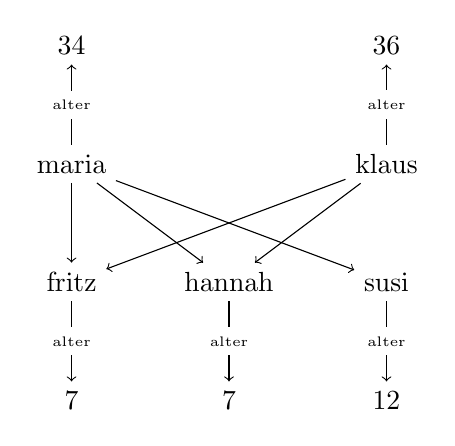
\begin{tikzpicture}
        \begin{scope}[every node/.style={fill=white}]
            \node (s1) at (0, 1.5) {maria};
            \node (s2) at (4, 1.5) {klaus};
            \node (s3) at (0, 0) {fritz};
            \node (s4) at (2, 0) {hannah};
            \node (s5) at (4, 0) {susi};
            \node (s6) at (0, 3) {34};
            \node (s7) at (4, 3) {36};
            \node (s8) at (0, -1.5) {7};
            \node (s9) at (2, -1.5) {7};
            \node (s10) at (4, -1.5) {12};
        \end{scope}
        \begin{scope}[every node/.style={fill=white}]
            \path [->] (s1) edge (s3);
            \path [->] (s1) edge (s4);
            \path [->] (s1) edge (s5);
            \path [->] (s2) edge (s3);
            \path [->] (s2) edge (s4);
            \path [->] (s1) edge node {\tiny{alter}} (s6);
            \path [->] (s2) edge node {\tiny{alter}} (s7);
            \path [->] (s3) edge node {\tiny{alter}} (s8);
            \path [->] (s4) edge node {\tiny{alter}} (s9);
            \path [->] (s5) edge node {\tiny{alter}} (s10);
        \end{scope}
    \end{tikzpicture}
    \end{center}
    (Unbeschriftete Kanten sind \enquote{kind}) 
    \begin{align*}
        {(\text{kind};\text{alter})}^\MI &= \{(\text{maria}, 7), (\text{maria},12), \ldots\}\\
        {(\exists \text{alter}.=_7)}^\MI &= \{\text{hannah}, \text{fritz}\}\\
        {(\forall \text{alter}.=_7)}^\MI &= \{\text{hannah}, \text{fritz}\}\\
        {(\exists \text{alter},\text{kind};\text{alter}.>)}^\MI &= \{\text{maria}, \text{klaus}\}\\
        {(\forall \text{alter},\text{kind};\text{alter}.>)}^\MI &= \Delta^\MI
    \end{align*}
\end{tafel}


Wir zeigen, dass bereits scheinbar einfache konkrete Bereiche zu Unentscheidbarkeit führen können. Betrachte $\MB_1$ mit:
\begin{align*}
    \Delta^{\MB_1} &= \mathbb{N}\\
    \Phi^{\MB_1} &= \{=_0, =, +_1\}
\end{align*}
wobei $=_0$ einstellig ist und $=, +_1$ zweistellig sind, mit den Extensionen:
\begin{align*}
    =_0^{\MB_1} &= \{0\}\\
    =^{\MB_1} &= \{(i, i) \mid i \in \mathbb{N} \}\\
    +_1^{\MB_1} &= \{(i, i + 1) \mid i \in \mathbb{N} \}\\
\end{align*}

\begin{theorem}
    Erfüllbarkeit von $\ALC(\MB_1)$-Konzepten bezüglich TBoxen ist \emph{unentscheidbar}.
\end{theorem}

Beweis per Reduktion des Halteproblems für 2-Registermaschinen.

\subsubsection{2-Registermaschinen}

2-Registermaschinen sind ähnlich Turingmaschinen:
\begin{itemize}
    \item Es gibt endlich viele Zustände.
    \item Statt eines Arbeitsbandes gibt es zwei Register mit Werten $\in \mathbb{N}$.
    \item Statt einer Übergangsfunktion gibt es Instruktionen.
\end{itemize}
Die Instruktionen erlauben es, den Wert eines Registers

\begin{itemize}
    \item zu inkrementieren oder
    \item auf 0 zu testen und bei Wert $\neq 0$ zu dekrementieren.
\end{itemize}
Bei der zweiten Art Instruktion hängt der Folgezustand davon ab, ob der Registerwert 0 war.

\begin{definition}[2-Registermaschine]
(Deterministische) \emph{2-Registermaschine} (2RM) ist Paar
$M = \left( Q,P \right)$ mit
$Q = \left\{ q_0,\ldots,\ q_\ell \right\}$ Menge von \emph{Zuständen}
und $P = I_{0},\ldots,I_{\ell - 1}$ \emph{Instruktionsfolge}. Per
Definition ist $q_0$ Startzustand und $q_\ell$ Stoppzustand. Jede
Instruktion $I_{i}$ hat eine der folgenden Formen:

\begin{itemize}
\item
  $I_{i} = + (p,q_j)$ mit $p \in \left\{ 1,2 \right\}$
  \emph{Register} und $q_{j}$ Folgezustand: Inkrementierunsanweisung
\item
  $I_{i} = - (p,q_{j},q_{k})$ mit $p \in \left\{ 1,2 \right\}$
  Register und $q_{j},q_{k}$ Folgezustände: Dekrementierungsanweisung
  mit Folgezustand $q_{j}$, wenn Register $p$ den Wert $0$ enthält
  und $q_{k}$ sonst.
\end{itemize}
\end{definition}

\begin{definition}[2-Registermaschinenberechnung]

\end{definition}

\subsubsection{Definition 5.31}\label{definition-5.31}

Konfiguration und Konfigurationsübergänge
$\left( q,m,n \right) \vdash_{M}(q^{'},m',n^{'})$. Berechnung als
eindeutige längste Konfigurationsfolge.

\subsubsection{Theorem 5.29}\label{theorem-5.29}

Das Erfüllbarkeitsproblem in $ALC(B_1)$ ist unentscheidbar.

\begin{itemize}
\item
  $\Delta^{B_1}\mathbb{= N}$
\item
  $\Phi^{B_1} = \left\{ =_{0}, = , +_1 \right\}$, wobei $=_{0}$
  einstellig, die anderen Zweistellig.
\end{itemize}

Beweisskizze. Gegeben 2RM $M$,
konstuiere$\text {$\ALC$}\left( B_1 \right)$-TBox $T_{M}$ und wähle
einen Konzeptnamen $J$ sodass: $M$ hält auf $\left( 0,0 \right)$
gdw. $J$ unerfüllbar bzgl. $T_{M}$. Zeige dies jeweils für
Hinrichtung und Rückrichtung per Kontraposition. \textbf{Wo kommen i und
j her?}
